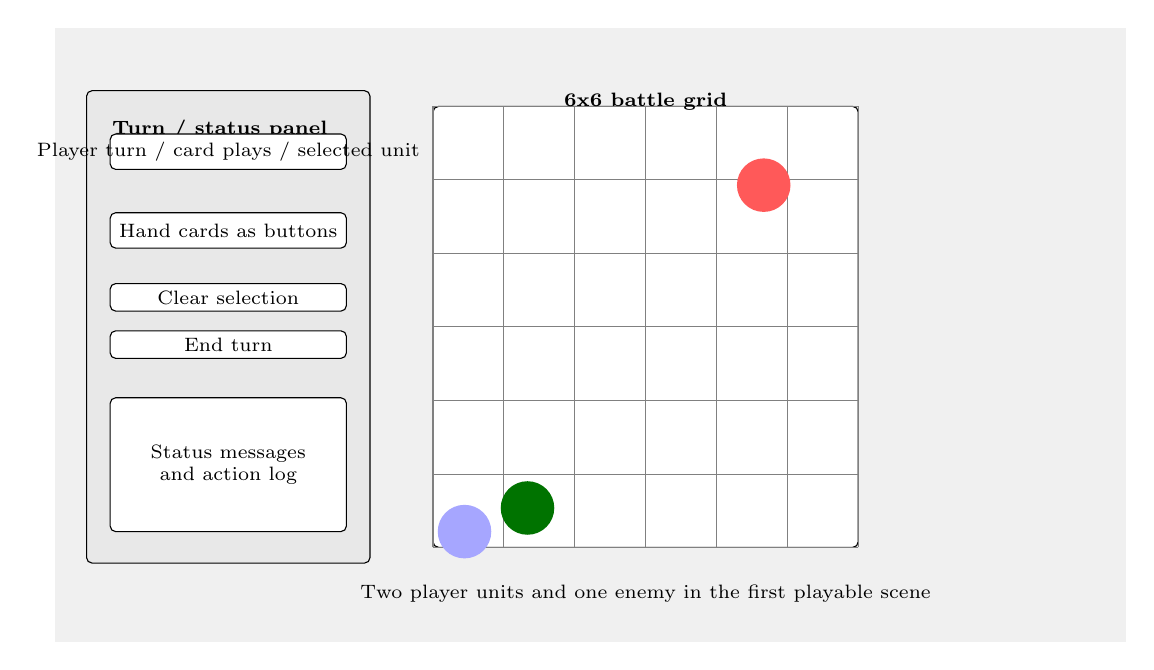
\begin{tikzpicture}[
    x=1cm,
    y=1cm,
    font=\scriptsize,
    panel/.style={draw, rounded corners=2pt, fill=gray!8},
    note/.style={draw, rounded corners=2pt, fill=white, align=center}
]
\fill[gray!12] (0,0) rectangle (13.6,7.8);

\draw[panel, fill=gray!18] (0.4,1.0) rectangle (4.0,7.0);
\node[anchor=north west] at (0.6,6.75) {\textbf{Turn / status panel}};
\draw[note] (0.7,6.0) rectangle (3.7,6.45);
\node at (2.2,6.22) {Player turn / card plays / selected unit};
\draw[note] (0.7,5.0) rectangle (3.7,5.45);
\node at (2.2,5.22) {Hand cards as buttons};
\draw[note] (0.7,4.2) rectangle (3.7,4.55);
\node at (2.2,4.37) {Clear selection};
\draw[note] (0.7,3.6) rectangle (3.7,3.95);
\node at (2.2,3.77) {End turn};
\draw[note] (0.7,1.4) rectangle (3.7,3.1);
\node[text width=2.5cm, align=center] at (2.2,2.25) {Status messages\\and action log};

\draw[panel, fill=white] (4.8,1.2) rectangle (10.2,6.8);
\foreach \x in {4.8,5.7,6.6,7.5,8.4,9.3,10.2} {
    \draw[gray] (\x,1.2) -- (\x,6.8);
}
\foreach \y in {1.2,2.13,3.07,4.0,4.93,5.87,6.8} {
    \draw[gray] (4.8,\y) -- (10.2,\y);
}
\node[anchor=north] at (7.5,7.1) {\textbf{6x6 battle grid}};
\fill[blue!35] (5.2,1.4) circle (0.34);
\fill[green!45!black] (6.0,1.7) circle (0.34);
\fill[red!65] (9.0,5.8) circle (0.34);
\node[anchor=north] at (7.5,0.85) {Two player units and one enemy in the first playable scene};
\end{tikzpicture}
